\section{Desarrollo}

\subsection{kNN}

El algorimo kNN (k Nearest Neighbours) se basa en el análisis de un conjunto de puntos del espacio para determinar a qué clase corresponde el nuevo objeto. En este caso cada imagen estará representada como un vector donde cada elemento es un píxel distinto de la misma. El conjunto de puntos elegido serán aquellas $k$ imágenes que más cerca se encuentren de la imagen a clasificar. Se clasificará a la nueva imagen como perteneciente a la clase que mayor representantes tenga en este conjunto de puntos cercanos.

Este algoritmo puede ser sumamente costoso en cuanto al tiempo de cómputo, y si la dimensión de los puntos a clasificar es muy grande, hacer uso del mismo podría resultar impracticable. Es por esto que se implementó un método cuyo objetivo es preprocesar las imágenes para reducir la cantidad de dimensiones de las muestras, permitiendo a kNN trabajar con muestras de una menor cantidad de variables. Este método es conocido como PCA (Principal components analysis).

\subsection{PCA}

El método de análisis de componentes principales se encarga de cambiar de base el conjunto de datos de entrada para obtener una mejor representación de los datos, y además reduce la dimensión de cada elemento tanto como se desee. Al reducir la dimensión de un punto es claro que se pierde información sobre el mismo, pero la particularidad de este método es que, se queda con las componentes más importantes, dejando de lado las que menos información aporten (de allí su nombre). De este modo, la información que descartada es la de menor relevancia, por lo que se lo considera una buena manera de reducir el espacio de la entrada.

Es importante aclarar que el método no solamente reduce la dimensión de los datos, sino que cambia la base de los mismos. Si se utiliza el método para reducir la entrada de kNN, es necesario cambiar a la misma base la imagen a clasificar, de lo contrario estarían comparándose elementos pertenecientes a distintos espacios.

\bigskip

Procedimiento para el cambio de base:

\begin{enumerate}
\item Se define una base de datos de entrenamiento (para $kNN$) como el conjunto $\D = \{x_i : i = 1, . . . , n\}$.
\item Sea $\mu = (x_1 + ... + x_n)/n$ el promedio de las imágenes de $D = \{x_i : i = 1, ..., n\}$ tal que $x_i\in\mathbb{R}^{m}$. Definimos $X\in\mathbb{R}^{nxm}$ como la matriz que contiene en la $i$-ésima fila al vector $(x_i - \mu)^t/  \sqrt{n-1}$. La matriz de covarianza de la muestra $X$ se define como $M = X^t X$
\item Se calcula $X$ y con ella $M$.
\item Se calculan los autovectores de $M$ mediante el método de las potencias, con deflación. Cómo cada iteración en la que calculamos el autovector de la matriz en cuestión, este está asociado al autovalor de máximo módulo, los autovectores que habremos calculado se encontrarán ordenados por relevancia. De esta manera se calculan tan solo $\alpha$ autovectores, con $1 \leq \alpha \leq n$, siendo $\alpha$ la dimensión a la que se quiere reducir las imágenes. 
\item Se contruye la matriz $V$ con los autovectores calculados previamente, dispuestos como columnas. $V$ es la matriz de cambio de base.
\item Por último, se reduce la dimensión de $X$ cambiando su base. El resultado final es $V^tX^t$ que contiene la misma cantidad de imágenes pero expresadas en otra base, y en lugar de tener dimensión $n$, cada una tiene dimensión $\alpha$.
\end{enumerate}\tabularnewline

Es interesante notar que una vez hecho el cambio de base de las imágenes, éstas representan a las imágenes pero si se trata de graficarlas se obtendrá algo muy distinto a lo que era anteriormente y no podrá visualizarse nada en concreto. Solo volviendo a la base original sería posible, pero ya se habrá perdido mucha información por lo que probablemente sea difícil encontrarlo útil.

\subsection{Fotos y algorítmo Peola}

\begin{algorithm}[H]
\NoCaptionOfAlgo
	\KwData{	
	img, $\alpha$, $\sigma$ 
	\KwResult{La imagen manipulada}
	\caption{Deformación}
	\tcc{Generamos 2 matrices de desplazamiento aleatorias} 

	dx $\leftarrow$ rand(size(img))

	dy $\leftarrow$ rand(size(img))

	\tcc{Suavizamos con un filtro gausseano la aleatoriedad de la matriz}
	fdx $\leftarrow$ $\alpha *$ imgaussfilt(dx, $\sigma$)

	fdy $\leftarrow$ $\alpha *$ imgaussfilt(dy, $\sigma$)

	\tcc{Aplica el desplazamiento aleatorio usando la interpolacion de griddata}
	res $\leftarrow$ griddata(fdx, fdy, img)
		}
\end{algorithm}

\begin{figure}[!htb]
\minipage{0.32\textwidth}
  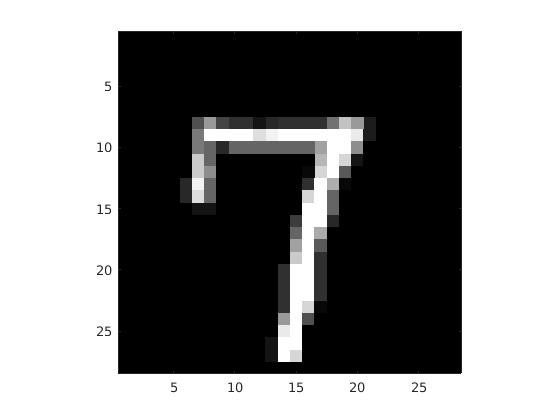
\includegraphics[width=\linewidth]{7original.jpg}
  \caption{Original}
\endminipage\hfill
\minipage{0.32\textwidth}
  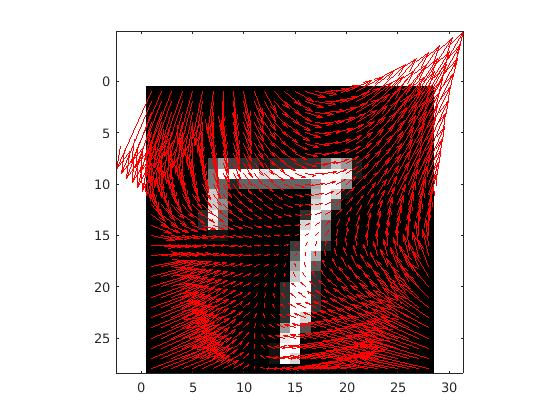
\includegraphics[width=\linewidth]{7vectpres.jpg}
  \caption{Vectores de desplazamiento}
\endminipage\hfill
\minipage{0.32\textwidth}%
  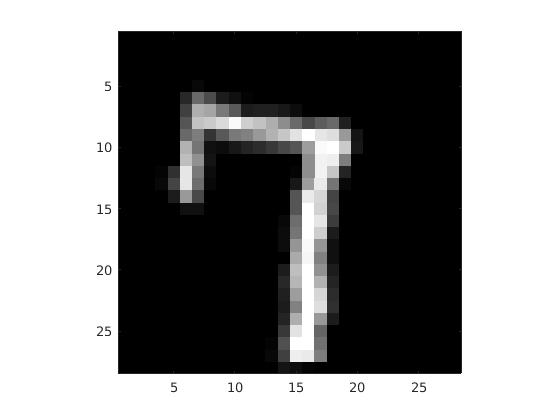
\includegraphics[width=\linewidth]{7resultado.jpg}
  \caption{Resultado}
\endminipage
\end{figure}


Como se puede observar, el dígito resultante es distinto al original pero al ojo humano sigue siendo el mismo dígito. Con este método generamos un nuevo data-set aplicando esta función a cada imagen y así ahora tenemos el doble de datos 84000 dígitos. 

Además de notar que los trazos no son perfectos, la orientación y rotación de los dígitos no es siempre la misma. Quisimos llevar al extremo aumentar los datos y aplicamos una segunda transformación a los dígitos. Para ello aplicamos una rotación aleatoria a cada dígito, usando la función de matlab para rotar imágenes imrotate, generamos un número aleatorio entre un cierto rango que le pasamos por parámetro como el ángulo. 30 grados nos pareció razonable ya que si se le aplica más hay dígitos que no se verían beneficiados.

\begin{figure}[ht] 
  \begin{minipage}[b]{0.5\linewidth}
    \centering
    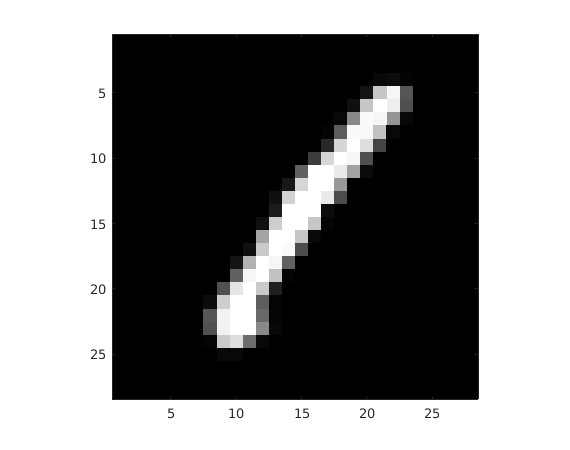
\includegraphics[width=.5\linewidth]{1_sinrotar.png} 
    \caption{Dígito Original 1} 
    \vspace{4ex}
  \end{minipage}%%
  \begin{minipage}[b]{0.5\linewidth}
    \centering
    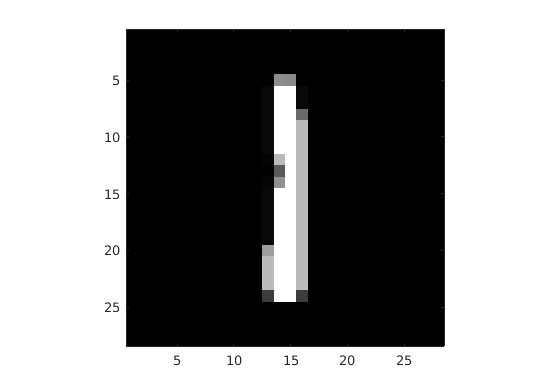
\includegraphics[width=.5\linewidth]{1_parecido.png} 
    \caption{Dígito Original 2} 
    \vspace{4ex}
  \end{minipage} 
  \begin{minipage}[b]{0.5\linewidth}
    \centering
    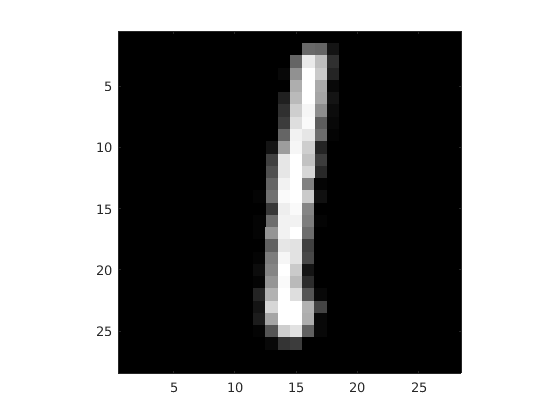
\includegraphics[width=.5\linewidth]{1_rot30.png} 
    \caption{Dígito 1 rotado $30^\circ$ sentido horario} 
    \vspace{4ex}
  \end{minipage}%% 
  \begin{minipage}[b]{0.5\linewidth}
    \centering
    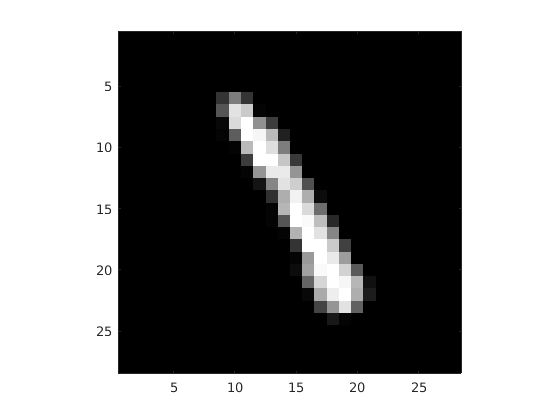
\includegraphics[width=.5\linewidth]{1_chueco.png} 
    \caption{Dígito 2 rotado $30^\circ$ sentido horario} 
    \vspace{4ex}
  \end{minipage} 
\end{figure}


\subsection{$X^t*X$ y $X*X^t$}
El método de la potencia con deflación se utiliza para obtener tanto los autovectores como los valores asociados de una matríz. Éste método es particualarmente suceptible al tamaño de la matríz que entra como parámetro. Al ser $X\in\mathbb{R}^{nxm}$ (con $m >> n$), la matríz $M$ acarrea un gran costo temporal para el cómputo del método de la potencia con deflación. Por lo que definimos la matríz $\^{M}\in\mathbb{R}^{nxn}$ como $\^{M}=X*X^t$. Como podemos ver, $\^{M}$ depende de la cantidad de imágenes de training set (que tiene como cota superior 410), por lo que será mucho más chica que $M$. Propondremos un método que utiliza los autovectores y autovalores de $\^{M}$ (cuyo cálculo implíca menor costo temporal) para obtener los de $M$.

\\
Primero veamos que relación hay entre los autovectores y los autovalores de {$X^t*X$ y $X*X^t$}:\\
\begin{center}
Sea $X\in\mathbb{R}^{nxm}$, $\^{M}=XX^t$ y $M=X^tX$.\\
Sea $v_i$ el autovector de $\^{M}$ asociado a $\lambda_i$, para  $i = 1, ..., n$.\\
\Rightarrow $\^{M}v_i=\lambda_iv_i$, para  $i = 1, ..., n$. Por definición de autovalor y autovector.\\
\Rightarrow $XX^tv_i=\lambda_iv_i$. Porque $\^{M}=XX^t$. \\
\Rightarrow $X^tXX^tv_i=\lambda_iX^tv_i$. Multiplico a izquierda por $X^t$.\\
 Defino $u_i=X^tv_i$\\
\Rightarrow $X^tXu_i=\lambda_iu_i$\\
Como $M=X^tX$,\\
\Rightarrow$Mu_i = \lambda_iu_i$\\
\therefore $u_i$ es el autovector de $M$ asociado al autovalor $\lambda_i$
\end{center}\\
\bigskip

Procedimiento para obtener los autovectores y autovalores de $M$ a partir de  $\^{M}$ utilizando la definición de $u_i$ que acabamos de formular:
\begin{enumerate}
\item Utilizando el método de la potencia con deflación se calculan los autovectores y autovalores de $\^{M}=X*X^t$ ($v_i$ y $\lambda_i$, para  $i = 1, ..., n$). 
\item Se crea una matríz $V\in\mathbb{R}^{nxn}$ y en sus columnas se colocan los autovectores $v_i$ de $\^{M}$ en el orden que fueron apareciendo (el método de la potencia con deflación devuelve los autovectores ordenados por módulo y sus autovectores correspondientes). Se guardan aparte los $n$ autovalores $\lambda_i$,  $i = 1, ..., n$.
\item Se calcúla $U=X^t*V$, en cada columna $U$ tendrá $u_i = X^t*v_i$ para $i = 1, ..., n$.
\item Recorriendo las columnas de $U$ se recuperan los autovectores $u_i$ de $M$.

\end{enumerate}\tabularnewline


\subsection{Validación cruzada}
Dado que necesitamos conocer previamente a qué persona corresponde una imagen para
poder estimar la correctitud de la clasificación, una alternativa es particionar la base de
entrenamiento en dos, utilizando una parte de ella en forma completa para el entrenamiento
y la restante como test, pudiendo ası́ corroborar la clasificación realizada, al contar con el
etiquetado del entrenamiento. Sin embargo, realizar toda la experimentación sobre una única
partición de la base podrı́a resultar en una incorrecta estimación de parámetros, dando lugar
al conocido problema de overfitting.\\
Por lo tanto, se estudiará la técnica de $cross validation$, en particular el $K-fold cross
validation 1$ , para realizar una estimación de los parámetros de los métodos que resulte estadı́sticamente más robusta.\\


La validación cruzada \textit{K-fold} consiste en particionar la base de entrenamiento en $K$ partes del mismo tamaño. Luego se realiza $K$ iteraciones, cada una de ellas reteniendo uno de los conjuntos para validación y utilizando los restantes $K - 1s$ para entrenamiento. Este método usualmente permite tomar las particiones sin cuidado alguno, pero en nuestro caso de uso tal cosa no es conveniente. Esto se debe a que en nuestra base de entrenamiento cada persona está representada por diez imágenes, con lo cual dividir las muestras de forma aleatoria puede desbalancear que tan representadas estan algunas personas en el training set. Esto puede significar que el algoritmo se entrena poco para algunas personas y mucho para otras. Yendo más lejos, este desbalance en el train set siempre tiene su contraparte en el test set, impactando de forma negativa las métricas.
Para resolver este problema, se propuso el uso de un k-fold que respete las proporciones de imágenes de cada persona. Como el test set siempre tiene que tener la misma cantidad de fotos para cada persona. Como nuestro dataset cuenta con cuarenta y un personas diferentes, la cantidad de rows del test set será un multiplo de ese número. Esto implica que k será multiplo de diez. Se realizó un shuffle de las imágenes y se eligieron los folds respetando las proporciones mencionadas.

